\documentclass{standalone}

\usepackage{avant}
\renewcommand{\familydefault}{\sfdefault}

\usepackage{tikz}
\usetikzlibrary{mindmap}
\colorlet{first}{red!50}
\colorlet{second}{orange!50}
\colorlet{third}{blue!50}

\begin{document}
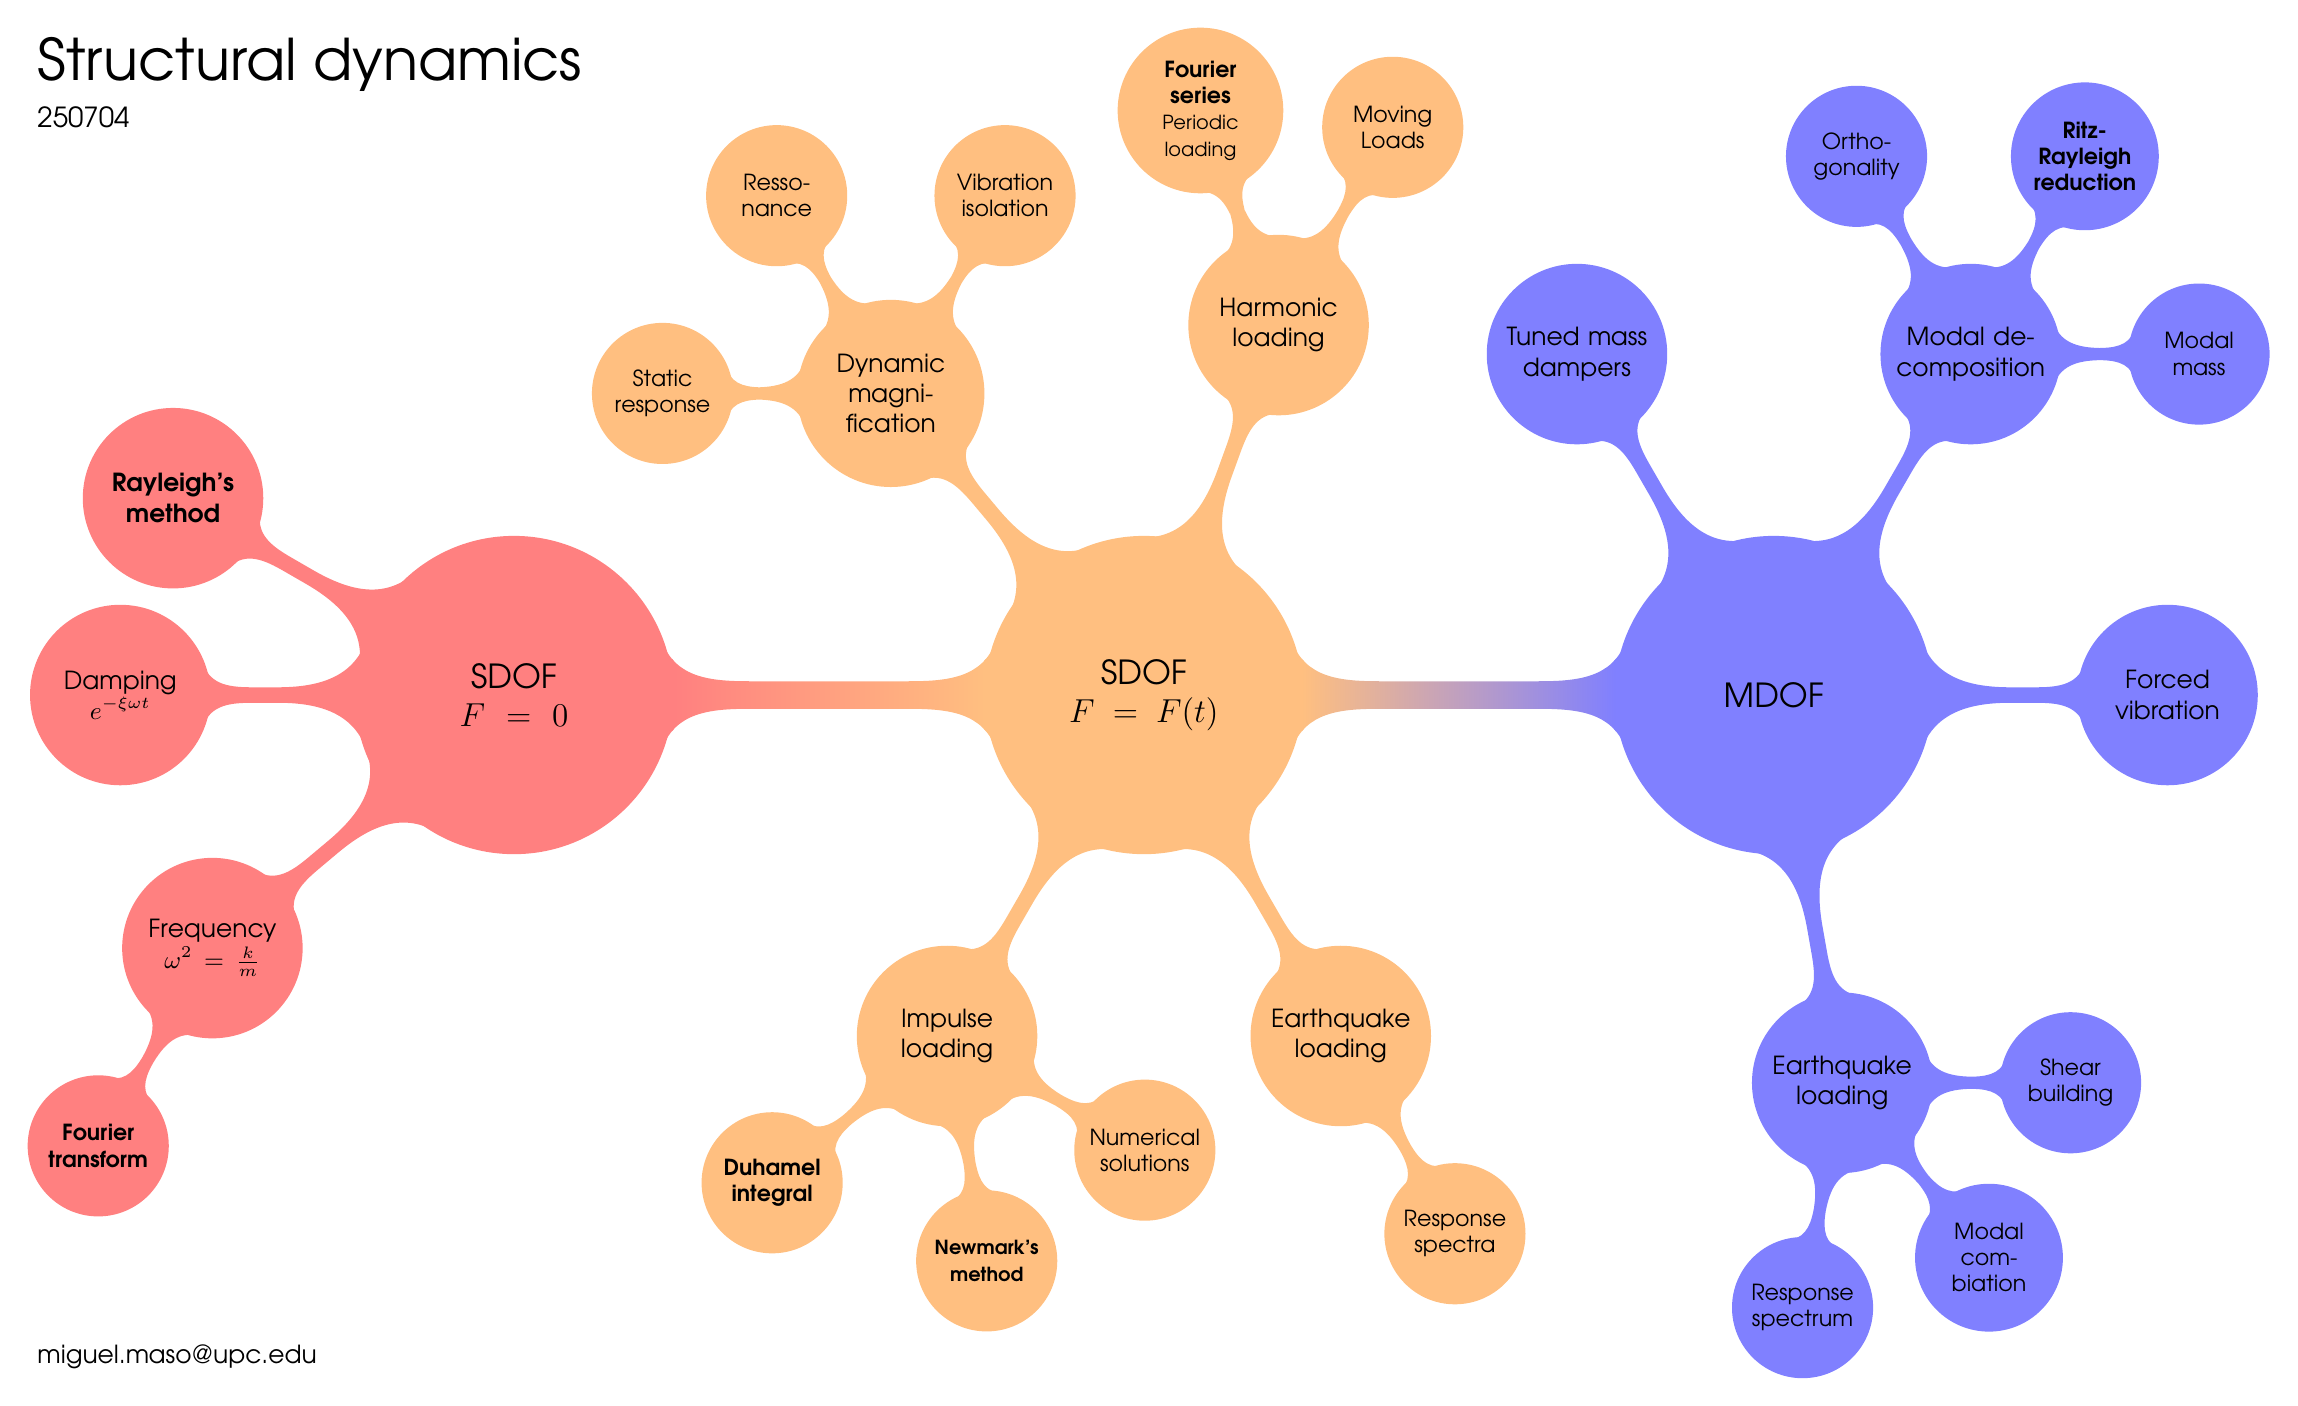
\begin{tikzpicture}

\path [mindmap,concept color=first] node [concept] (a) at (0,0) {SDOF\\$F=0$}
    child [grow=220] {node [concept] {Frequency $\omega^2=\frac{k}{m}$}
        child [grow=240] {node [concept] {\textbf{Fourier transform}}}
    }
    child [grow=180] {node [concept] {Damping $e^{-\xi\omega t}$}}
    child [grow=150] {node [concept] {\textbf{Rayleigh's method}}}
;
\path [mindmap,concept color=second] node [concept] (b) at (8,0){SDOF\\$F=F(t)$}
    child [grow=130] {node [concept] {Dynamic magnification}
        child [grow=180] {node [concept] {Static response}}
        child [grow=120] {node [concept] {Resso-\\nance}}
        child [grow=60]  {node [concept] {Vibration isolation}}
    }
    child [grow=70] {node [concept] {Harmonic loading}
        child [grow=60]  {node [concept] {Moving Loads}}
        child [grow=110] {node [concept] {\textbf{Fourier series}\\ \scriptsize{Periodic loading}}}
    }
    child [grow=240] {node [concept] {Impulse loading}
        child [grow=220] {node [concept] {\textbf{Duhamel integral}}}
        child [grow=280] {node [concept] {\scriptsize\textbf{Newmark's method}}}
        child [grow=330] {node [concept] {Numerical solutions}}
    }
    child [grow=300] {node [concept] {Earthquake loading}
        child [grow=300] {node [concept] {Response spectra}}
    }
;
\path [mindmap,concept color=third] node [concept] (c) at (16,0) {MDOF}
    child [grow=120] {node [concept] {Tuned mass dampers}}
    child [grow=60]  {node [concept] {Modal decomposition}
        child [grow=120] {node [concept] {Ortho-\\gonality}}
        child [grow=60]  {node [concept] {\textbf{Ritz-Rayleigh reduction}}}
        child [grow=0]   {node [concept] {Modal mass}}
    }
    child [grow=0]   {node [concept] {Forced vibration}}
    child [grow=280] {node [concept] {Earthquake loading}
        child [grow=260] {node [concept] {Response spectrum}}
        child [grow=310]   {node [concept] {Modal combiation}}
        child [grow=0]  {node [concept] {Shear building}}
    }
;

\path (a) to[circle connection bar switch color=from (first) to (second)] (b);
\path (b) to[circle connection bar switch color=from (second) to (third)] (c);

\node at (current bounding box.north west) [anchor=north west,align=left] {\huge{Structural dynamics}\\[5pt]250704};
\node at (current bounding box.south west) [anchor=south west] {\small{miguel.maso@upc.edu}};

\end{tikzpicture}
\end{document}
